\paragraph{QuizziPedia::Back-End::App::Models::QuestionModel}
\label{QuizziPedia::Back-End::App::Models::QuestionModel}
\begin{figure}[ht]
	\centering
	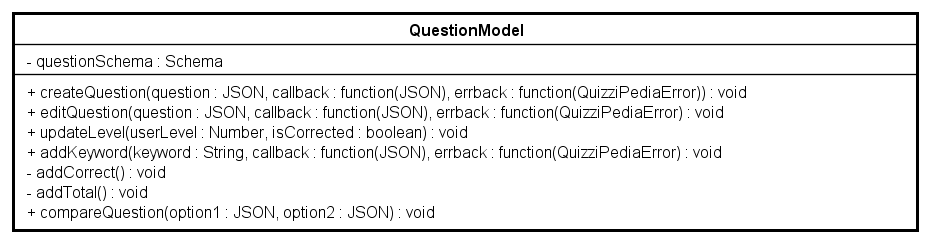
\includegraphics[scale=0.45]{UML/Classi/Back-End/QuizziPedia_Back-End_App_Models_questionModel.png}
	\caption{QuizziPedia::Back-End::App::Models::QuestionModel}
\end{figure}
\FloatBarrier
	\begin{itemize}
		\item \textbf{Descrizione} \\
		Classe che modella i dati relativi alle domande all'interno dell'applicazione;	
		\item \textbf{Utilizzo} \\
		Viene utilizzata per rappresentare le domande. Si interfaccia alla libreria \textit{Mongoose\ped{G}} per la creazione dello schema e dei relativi metodi statici o di istanza;
		\item \textbf{Relazione con altra classi}:
			\begin{itemize}
			\item \textbf{IN \texttt{UserModel}} \\
			Classe che rappresenta tutti gli utenti;
			\item \textbf{OUT \texttt{SummaryModel} }\\
			Classe che rappresenta i riepiloghi dei questionari svolti;
			\item \textbf{OUT \texttt{TopicModel}} \\
			Classe che rappresenta gli argomenti;
			\item \textbf{OUT \texttt{QuizModel}} \\
			Classe che modella i questionari all'interno dell'applicazione;
			\item \textbf{IN \texttt{QuestionController}} \\
			Classe che gestisce la logica applicativa riguardante la visualizzazione, la creazione e la modifica delle domande presenti nell'applicazione;
			\item \textbf{OUT \texttt{UserModel}} \\
			Classe che modella la creazione e la gestione dei dati utente;
			\item \textbf{IN \texttt{QuizModel}} \\
			Classe che modella i questionari all'interno dell'applicazione.
			\item \textbf{OUT \texttt{SummaryModel}} \\
			Classe che modella i riepiloghi all'interno dell'applicazione.
			\item \textbf{IN \texttt{TopicModel}} \\
			Classe che modella gli argomenti all'interno delle domande.
			\end{itemize}
		\item \textbf{Attributi}:
	\begin{itemize}
		\item \texttt{questionSchema: Schema} \\
		Questo campo dati rappresenta lo schema \textit{Mongoose\ped{G}} per le domande e prevede i seguenti attributi:
		\begin{itemize}
			\item \texttt{author} di tipo \texttt{ObjectId}, rappresenta il riferimento all'identificativo nel database dell'utente che ha creato la domanda;
			\item \texttt{makeWith} di tipo \texttt{String}, rappresenta con quale strumento è stata creata la domanda;
			\item \texttt{language} di tipo \texttt{String}, rappresenta la lingua in cui è scritta la domanda; 
			\item \texttt{question} di tipo \texttt{Array}, contiene un oggetto di tipo \texttt{JSON}. L'oggetto \texttt{JSON} è rappresentato dai seguenti campi:
				\begin{itemize}
					\item \texttt{questionText} di tipo \texttt{String}, rappresenta il testo della domanda; 
					\item \texttt{image} di tipo \texttt{String}, rappresenta l'\textit{URL\ped{G}} dell'immagine associata al testo della domanda; 
					\item \texttt{answers} di tipo \texttt{Array}, contiene un oggetto di tipo \texttt{JSON}. L'oggetto \texttt{JSON} è rappresentato dai seguenti campi:
					\begin{enumerate}	
						\item \texttt{type} di tipo \texttt{String}, rappresenta la tipologia di risposta; 				  
						\item \texttt{text} di tipo \texttt{String}, rappresenta il testo della risposta;
        					\item \texttt{url} di tipo \texttt{String}, rappresenta l'immagine della risposta;
        					\item \texttt{attributesForTForMultiple} di tipo \texttt{Mixed}, contiene i seguenti attributi:
        					\begin{enumerate}
        						\item \texttt{isItRight} di tipo \texttt{Boolean}, rappresenta se una risposta è giusta o sbagliata.
						\end{enumerate}      
						\item \texttt{attributesForSorting} di tipo \texttt{Mixed}, contiene i seguenti attributi:
        					\begin{enumerate}
        						\item \texttt{position} di tipo \texttt{Boolean}, rappresenta quale è la giusta posizione di un testo o immagine all'interno di un esercizio di ordinamento.
						\end{enumerate}  
							\item \texttt{attributesForLinking} di tipo \texttt{Mixed}, contiene i seguenti attributi:
        					\begin{enumerate}
        						\item \texttt{text1} di tipo \texttt{String}, rappresenta il primo elemento testuale che deve essere collegato con il secondo elemento testuale o rappresentato da un'immagine.
        						\item \texttt{text2} di tipo \texttt{String}, rappresenta il secondo elemento testuale che deve essere collegato con il primo elemento testuale o rappresentato da un'immagine.
        						\item \texttt{url1} di tipo \texttt{String}, rappresenta il primo elemento rappresentato da un'immagine che deve essere collegato con il secondo elemento testuale o rappresentato da un'immagine.
        						\item \texttt{url2} di tipo \texttt{String}, rappresenta il secondo elemento rappresentato da un'immagine che deve essere collegato con il primo elemento testuale o rappresentato da un immagine.
						\end{enumerate}  
							\item \texttt{attributesForClickableArea} di tipo \texttt{Mixed}, contiene i seguenti attributi:
        					\begin{enumerate}
        						\item \texttt{x} di tipo \texttt{Number}, rappresenta la coordinata x di una area cliccabile.  
        						\item \texttt{y} di tipo \texttt{Number}, rappresenta la coordinata y di una area cliccabile.  
						\end{enumerate}    
							\item \texttt{attributesForEmptySpaces} di tipo \texttt{Mixed}, contiene i seguenti attributi:
        					\begin{enumerate}
        						\item \texttt{wordNumber} di tipo \texttt{Number}, rappresenta la posizione dello spazio vuoto in cui deve andare inserita la parola.  
						\end{enumerate}        						  						
					\end{enumerate}
				\end{itemize}			
					\item \texttt{keywords} di tipo \texttt{Array}, contiene oggetti di tipo \texttt{String} che rappresentano le parole chiave utili per ricercare una domanda;	 
			\item \texttt{level} di tipo \texttt{Number}, rappresenta la difficoltà della domanda;
			\item \texttt{totalAnswers} di tipo \texttt{Number}, rappresenta le risposte totali che tutti gli utenti hanno dato alla domanda;
			\item \texttt{correctAnswers} di tipo \texttt{Number}, rappresenta quante risposte corrette hanno dato gli utenti che hanno risposto alla domanda.
		
		\end{itemize}
	\end{itemize}
\item \textbf{Metodi}:
	\begin{itemize}
	\item \texttt{+ createQuestion(question: JSON, callback: function(JSON),\\ errback: function(QuizziPediaError))} \\
	Metodo che permette la creazione di una nuova domanda; \\
		\textbf{Parametri}:
		\begin{itemize}
			\item \texttt{question: JSON} \\
			Rappresenta le informazioni che andranno a comporre la domanda da creare;
			\item \texttt{callback: function(JSON)} \\
			Rappresenta la \textit{callback\ped{G}} che verrà eseguita al termine dell'elaborazione nel caso non si verifichino errori durante l'esecuzione;
			\item \texttt{errback: function(QuizziPediaError)} \\
			Rappresenta la \textit{callback\ped{G}} che il metodo deve chiamare qualora si verificassero errori durante l'esecuzione del metodo.
		\end{itemize}   
	\item \texttt{+ editQuestion(question: JSON, callback: function(JSON),\\ errback: function(QuizziPediaError))} \\
	Metodo che permette di modificare una domanda già esistente; \\
		\textbf{Parametri}:
		\begin{itemize}
			\item \texttt{question : JSON} \\
			Rappresenta le nuove informazioni che andranno a modificare le informazioni precedenti di una specifica domanda;
			\item \texttt{callback: function(JSON)} \\
			Rappresenta la \textit{callback\ped{G}} che verrà eseguita al termine dell'elaborazione del metodo in caso non si verifichino errori durante l'esecuzione;
			\item \texttt{errback: function(QuizziPediaError)} \\
			Rappresenta la \textit{callback\ped{G}} che il metodo deve chiamare qualora si verificassero errori durante l'esecuzione del metodo.
		\end{itemize}
	\item \texttt{+ addKeyword(keyword: String, callback: function(JSON),\\ errback: function(QuizziPediaError))} \\
	Metodo che permette di aggiungere delle parole chiave ad una specifica domanda; \\
		\textbf{Parametri}:
			 \begin{itemize}
			 	\item \texttt{keyword: String} \\
			 	Rappresenta la parola chiave da inserire
			 	\item \texttt{callback: function(JSON)} \\
			 	Rappresenta la \textit{callback\ped{G}} che verrà eseguita al termine dell'elaborazione del metodo in caso si verifichino errori durante l'esecuzione;
			 	\item \texttt{errback: function(QuizziPediaError)} \\
			 	Rappresenta la \textit{callback\ped{G}} che il metodo deve chiamare qualora si verificassero errori durante l'esecuzione del metodo.
			 \end{itemize}
	\item \texttt{+ updateLevel(userLevel: Number, isCorrected: boolean)} \\
	Metodo che permette di aggiornare il livello di difficoltà della domanda, questo metodo è chiamato ogni qualvolta un utente risponde ad una domanda durante un allenamento;
		\textbf{Parametri}:
			\begin{itemize}
				\item \texttt{userLevel: Number} \\
				Indica, con un numero compreso tra 1 e 1000, l'abilità dell'utente che ha risposto alla domanda;
				\item \texttt{isCorrected: boolean} \\
				Indica se l'utente che ha risposto alla domanda ha risposto correttamente.
			\end{itemize}  
	\item \texttt{- addCorrect()} \\
	Metodo che permette di incrementare il contatore di risposte corrette di una determinata domanda;
	\item \texttt{- addTotal()} \\
	Metodo che permette di incrementare il contatore delle risposte date di una determinata domanda;
	\item \texttt{+ getQuestions(userID: ObjectId)}\\
	Metodo che ritorna tutte le domande create da un utente.\\
	\textbf{Parametri:}
	\begin{itemize}
		\item \texttt{userID: ObjectId}\\
		Rappresenta l'identificativo dell'utente del quale si vogliono ritornare le domande.
	\end{itemize}
	\end{itemize}
\end{itemize}
